\chapter{Flight Test}\label{chap:Flight}


\section{Flight Tests in the Vicon Room}

%\begin{figure}[H]
%   \centering
%   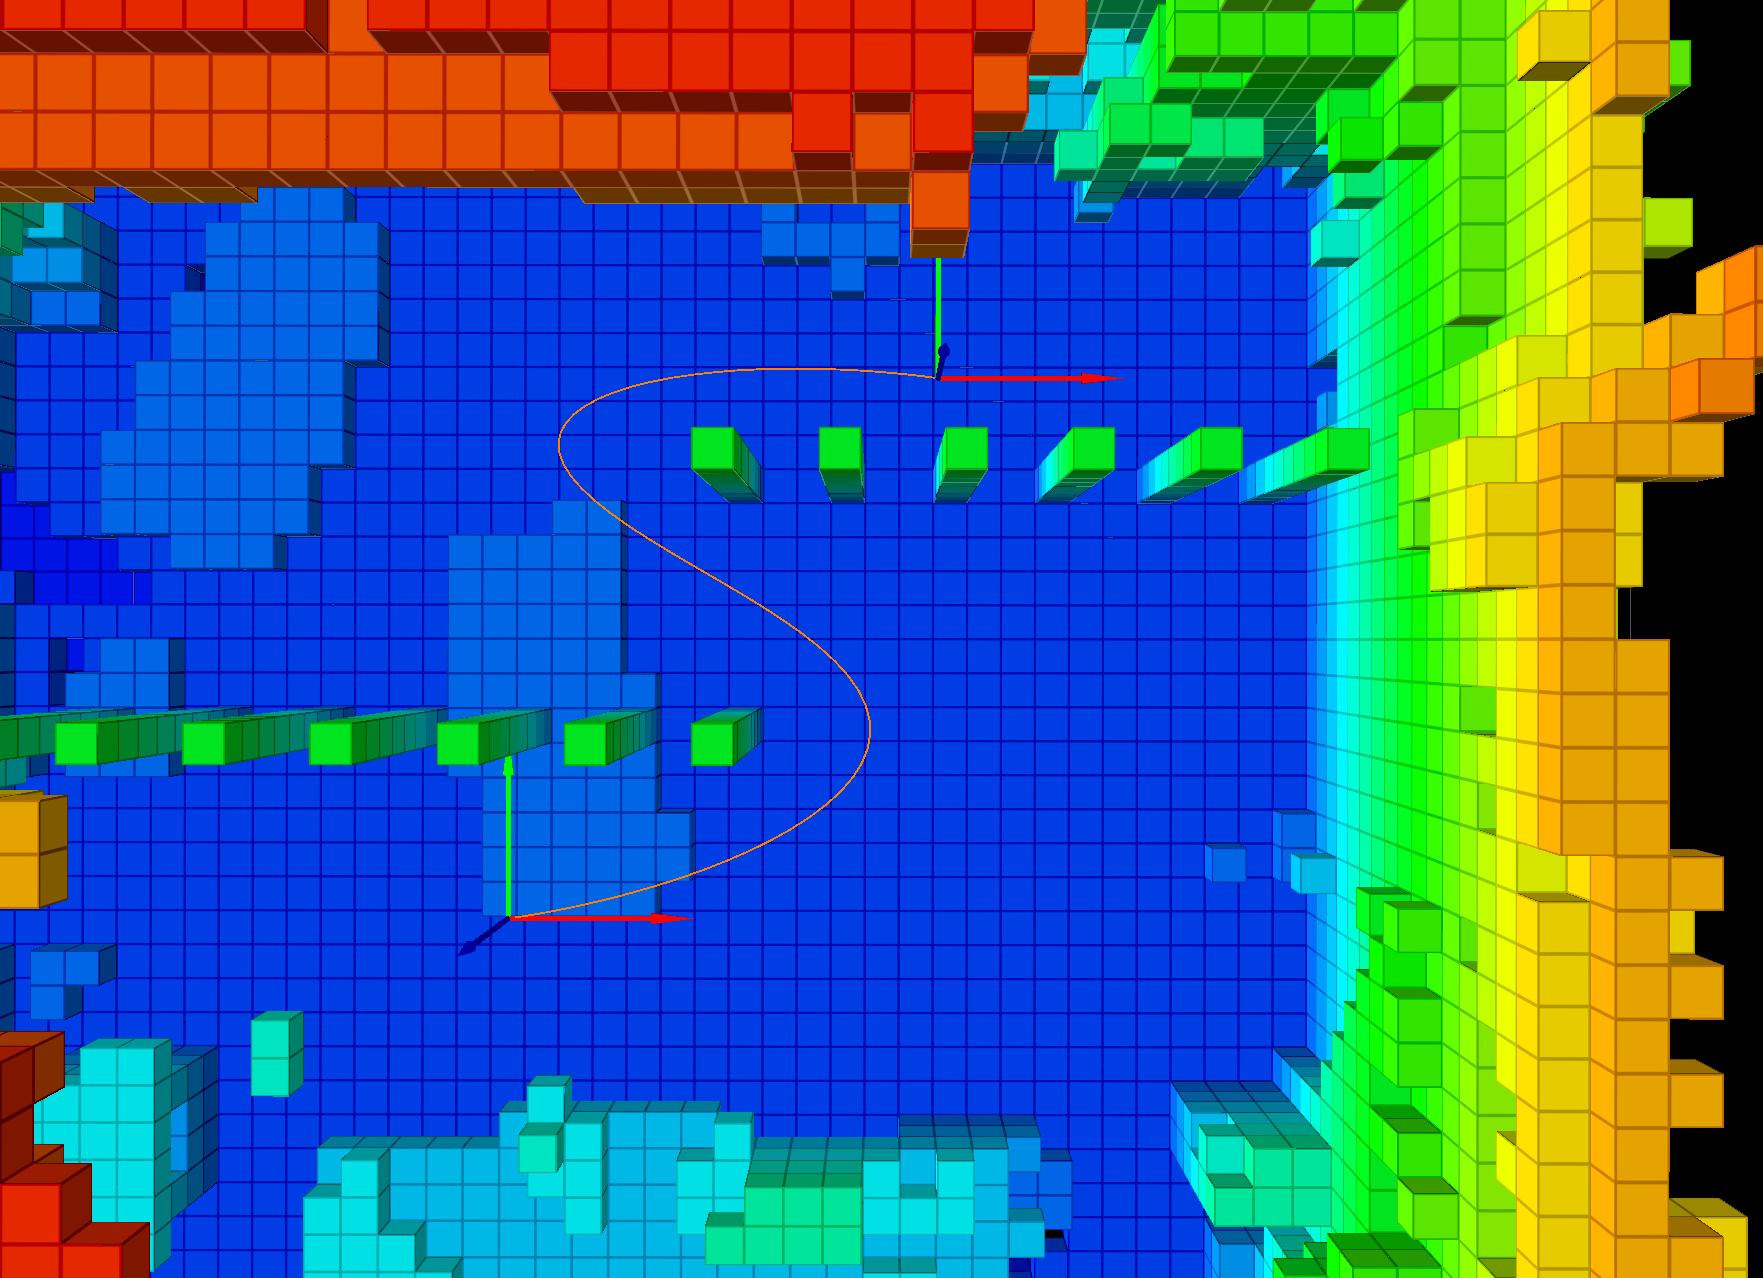
\includegraphics[trim = 0mm 0mm 0mm 0mm,clip,width=1\textwidth]{pics/2b.png}
%   \caption{Bird's eye perspective on hallways in the "ML" building of the ETH Zurich. One start vertex and 6 different goal vertices are depicted}
%   \label{pic:testsfgdsgfdf}
%\end{figure}


\begin{figure}[H]
   \centering
   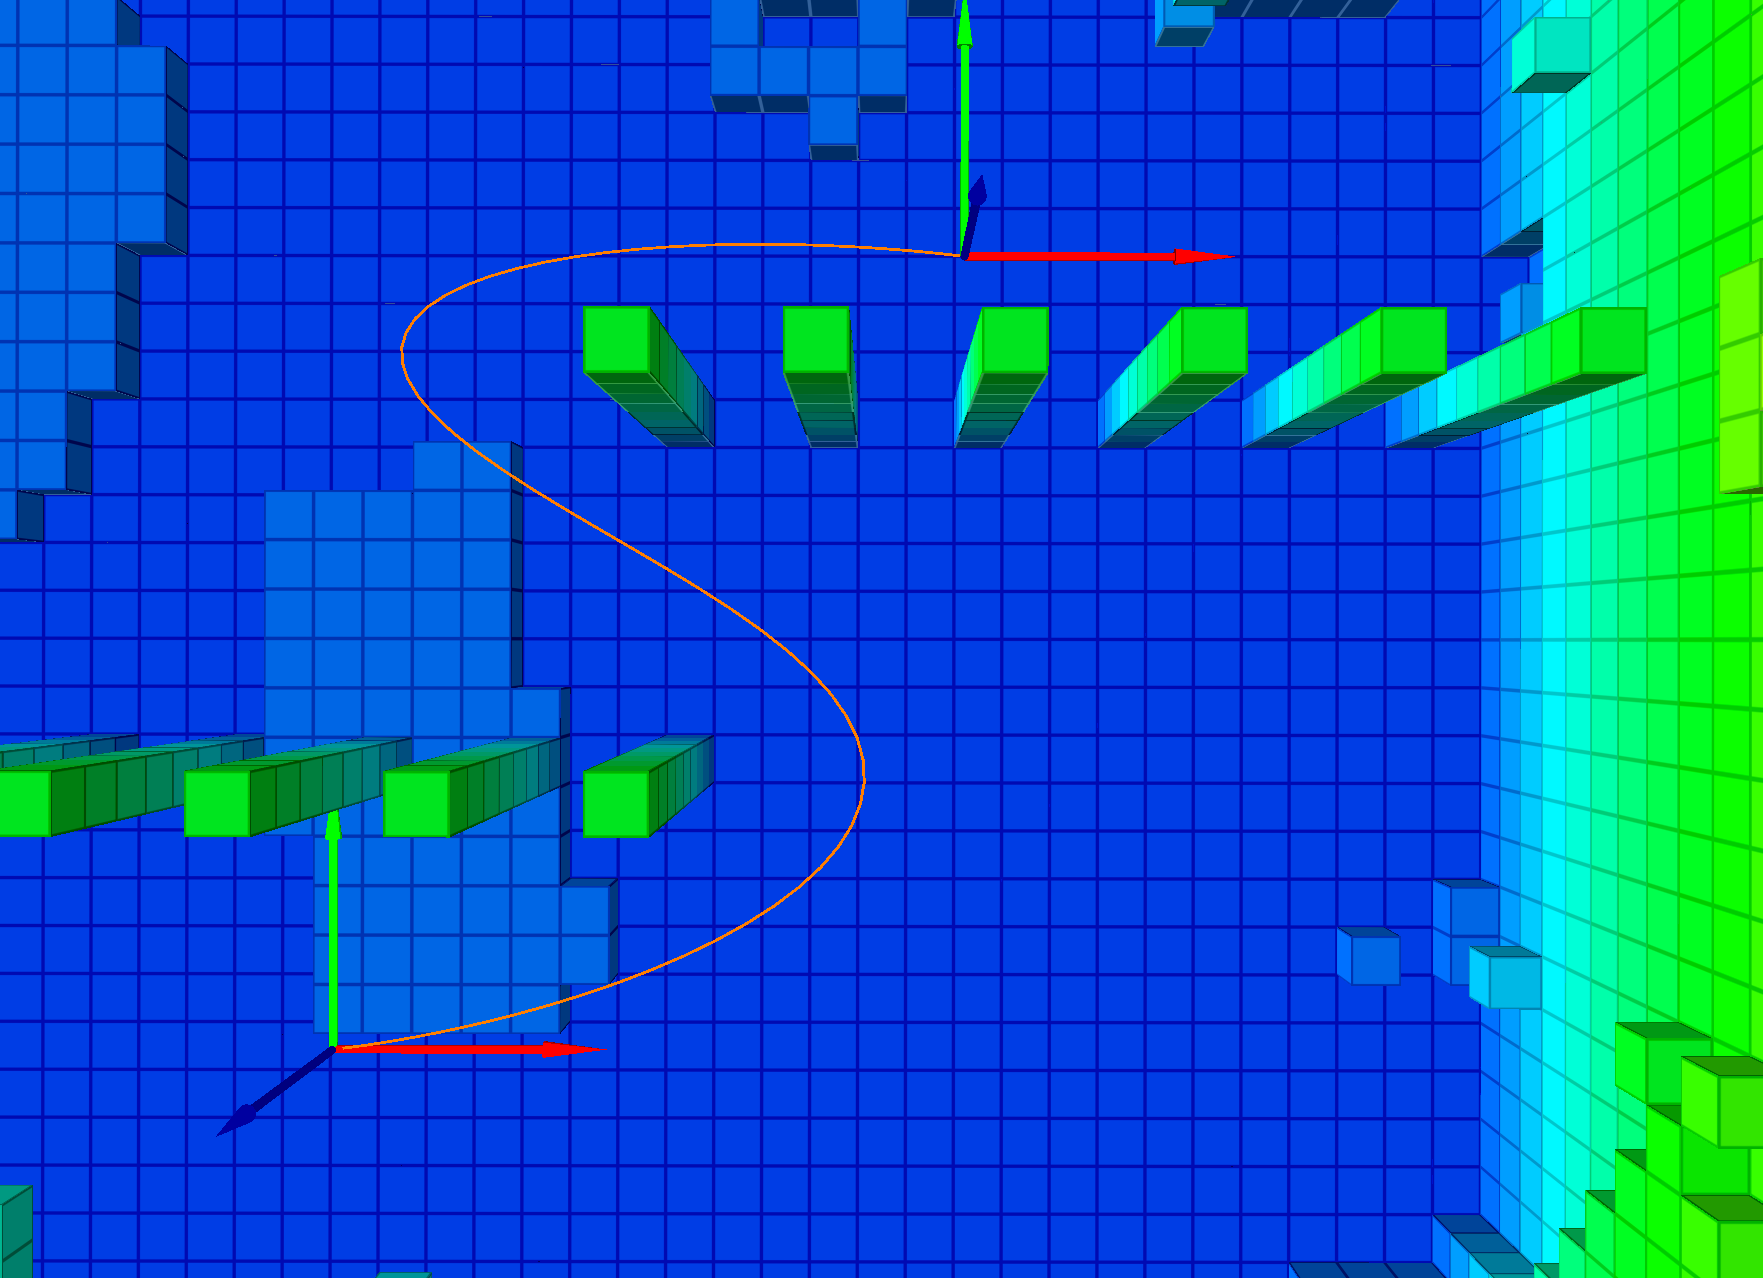
\includegraphics[trim = 0mm 0mm 0mm 0mm,clip,width=1\textwidth]{pics/2c.png}
   \caption{ein bild}
   \label{pic:testdfgd}
\end{figure}




\begin{figure}[H]
   \centering
   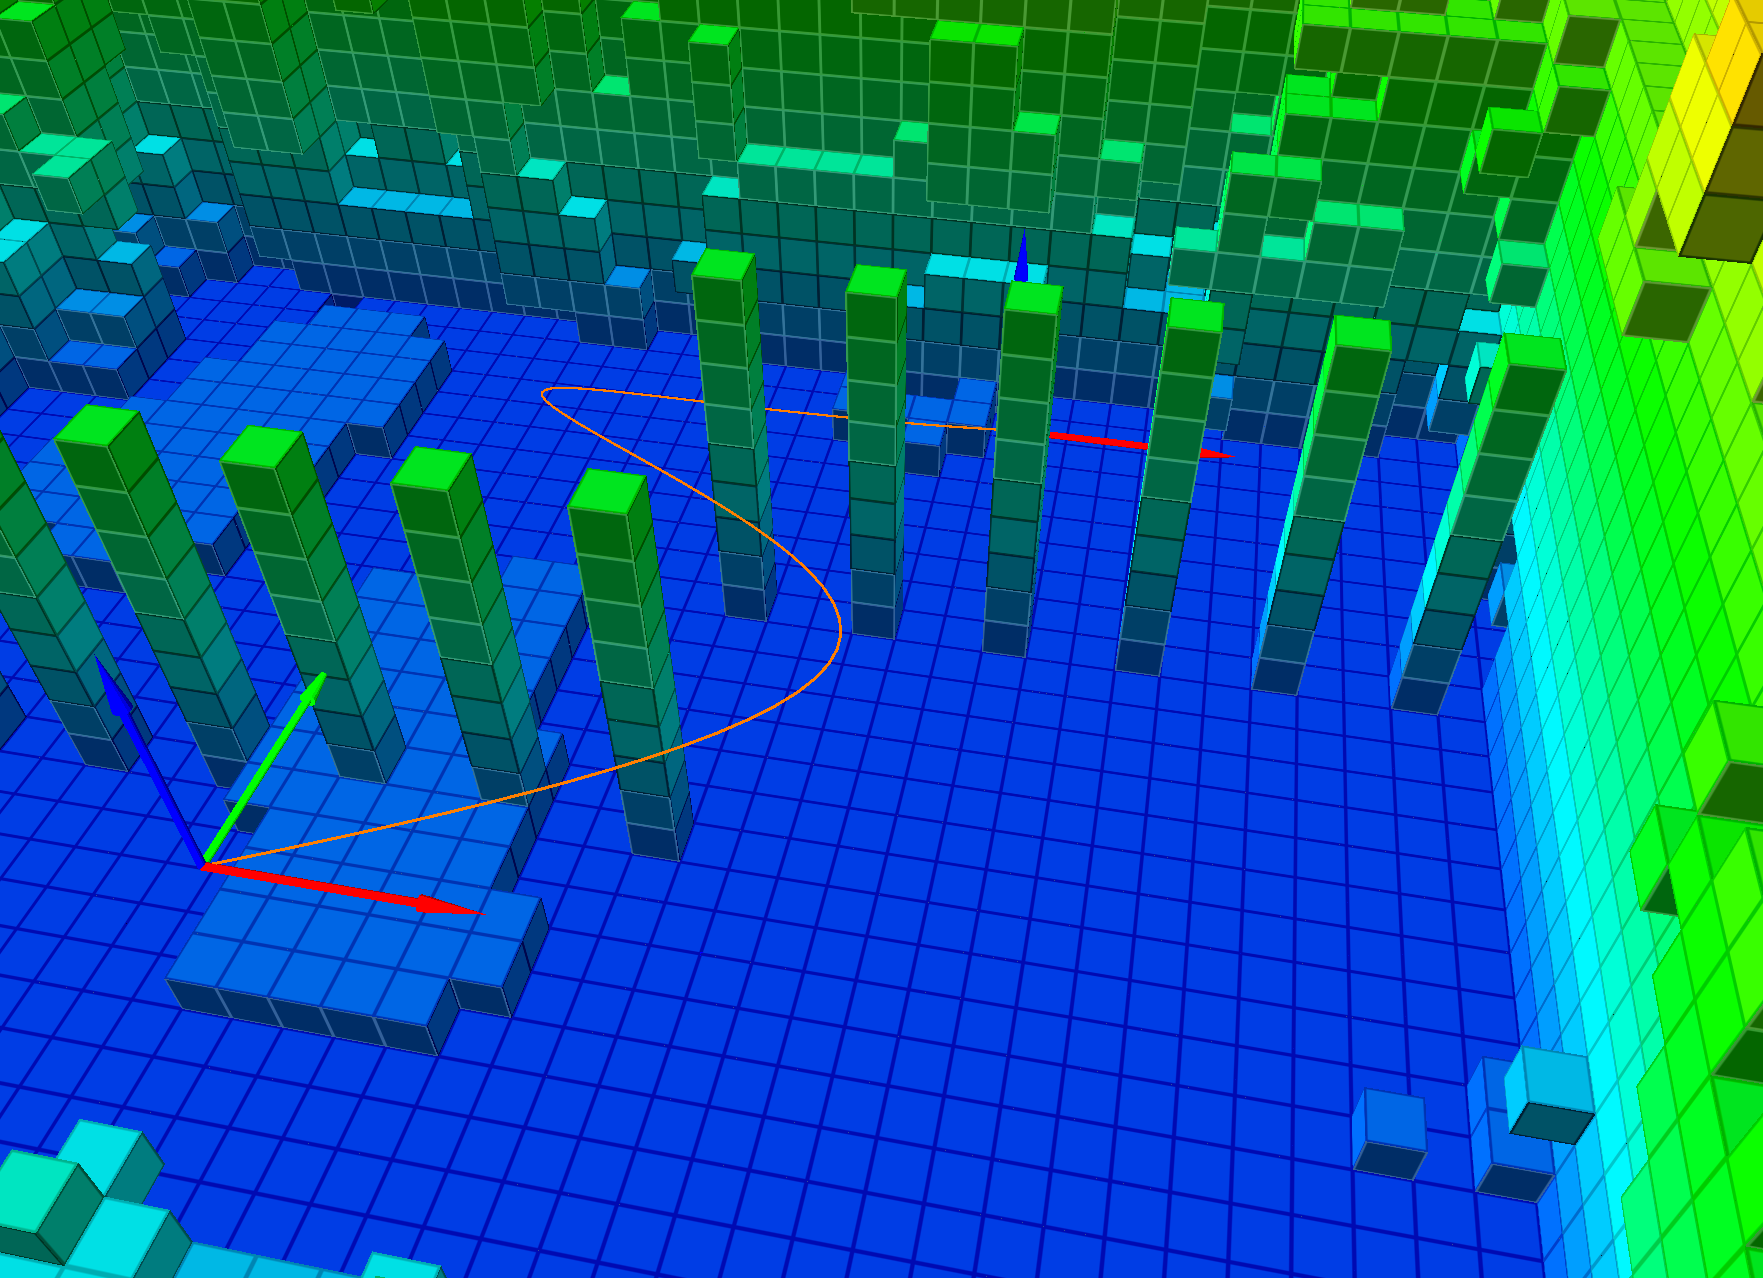
\includegraphics[trim = 0mm 0mm 0mm 0mm,clip,width=1\textwidth]{pics/2a.png}
   \caption{ein bild}
   \label{pic:testsfsfsdf}
\end{figure}



%\begin{figure}
%\centering
%\begin{subfigure}{.5\textwidth}
%  \centering
%  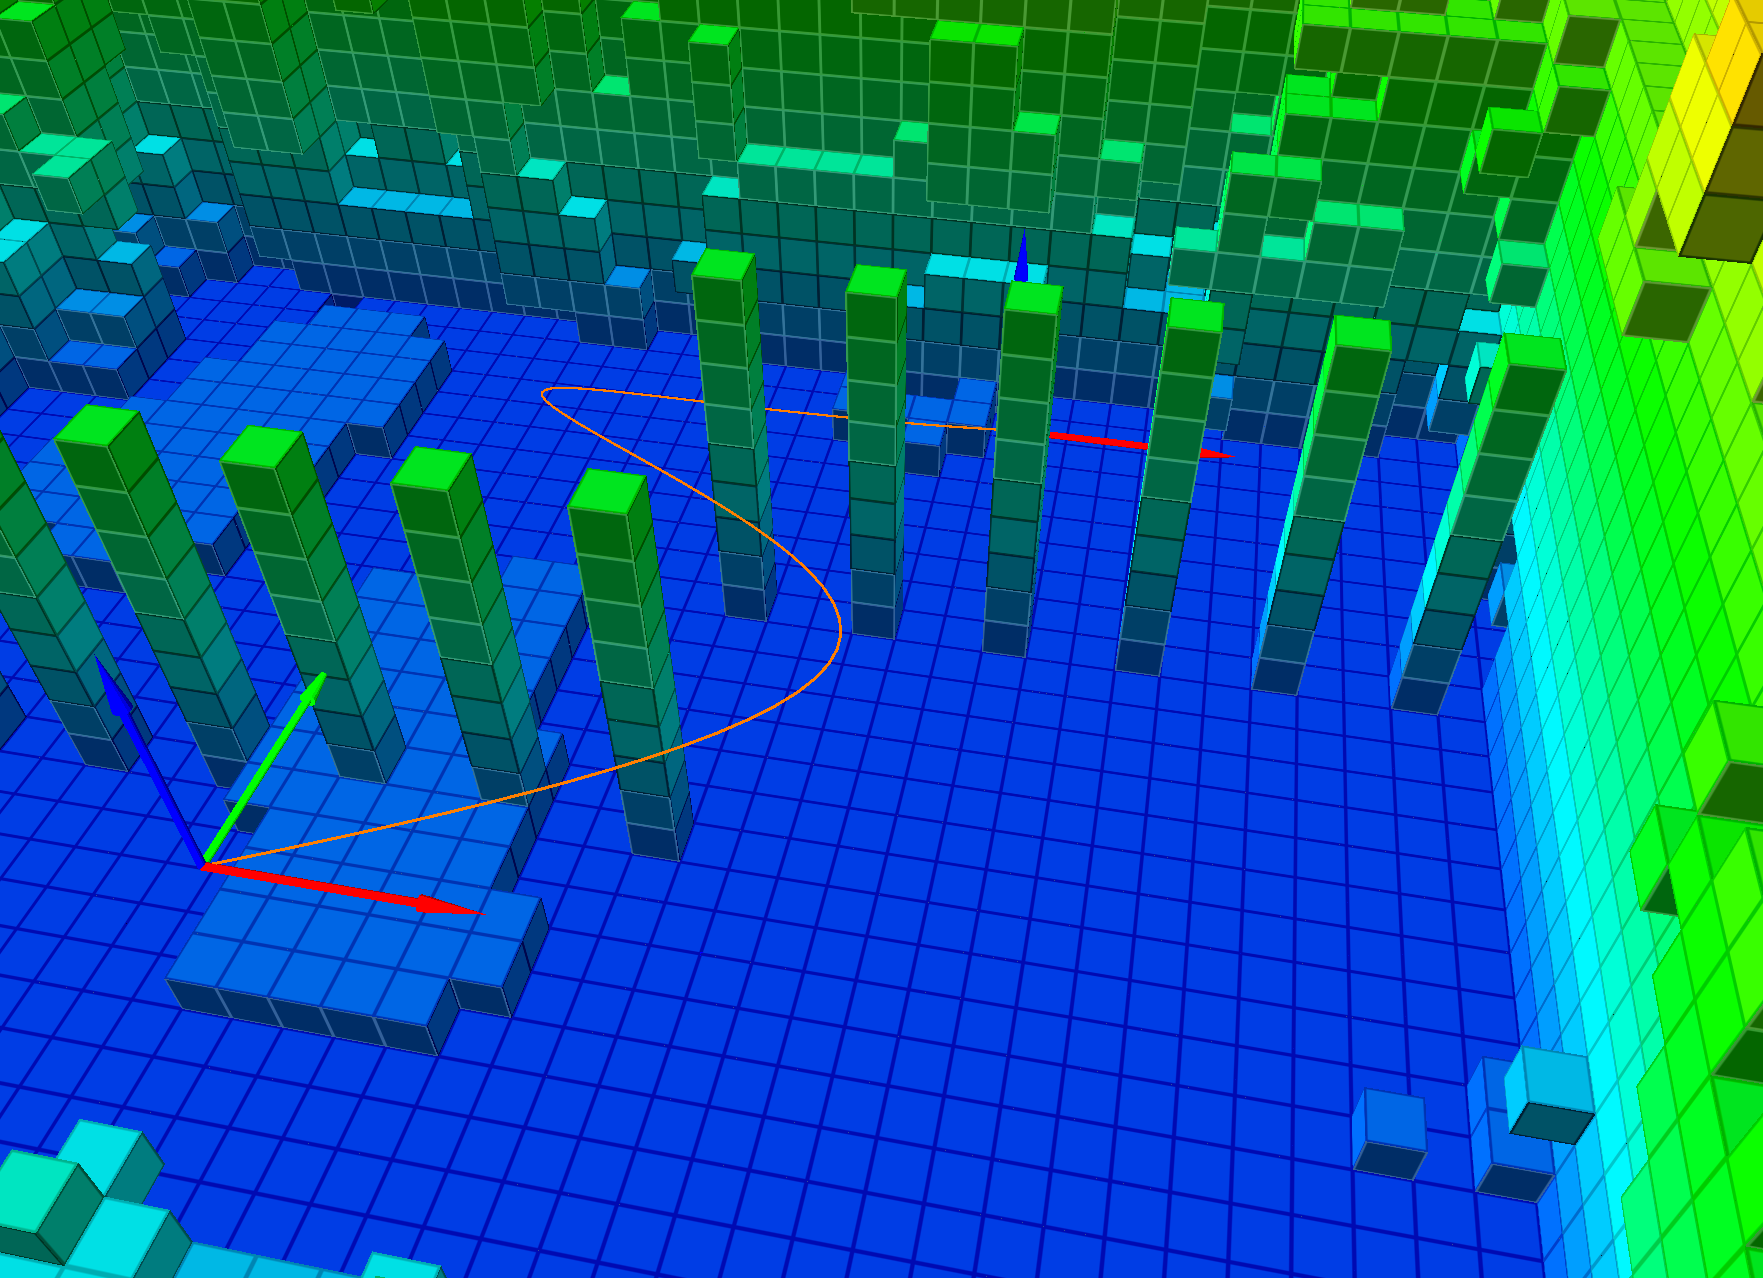
\includegraphics[width=1\linewidth]{pics/2a.png}
%  \caption{A subfigure}
%  \label{fig:sub1}
%\end{subfigure}%
%\begin{subfigure}{.5\textwidth}
%  \centering
%  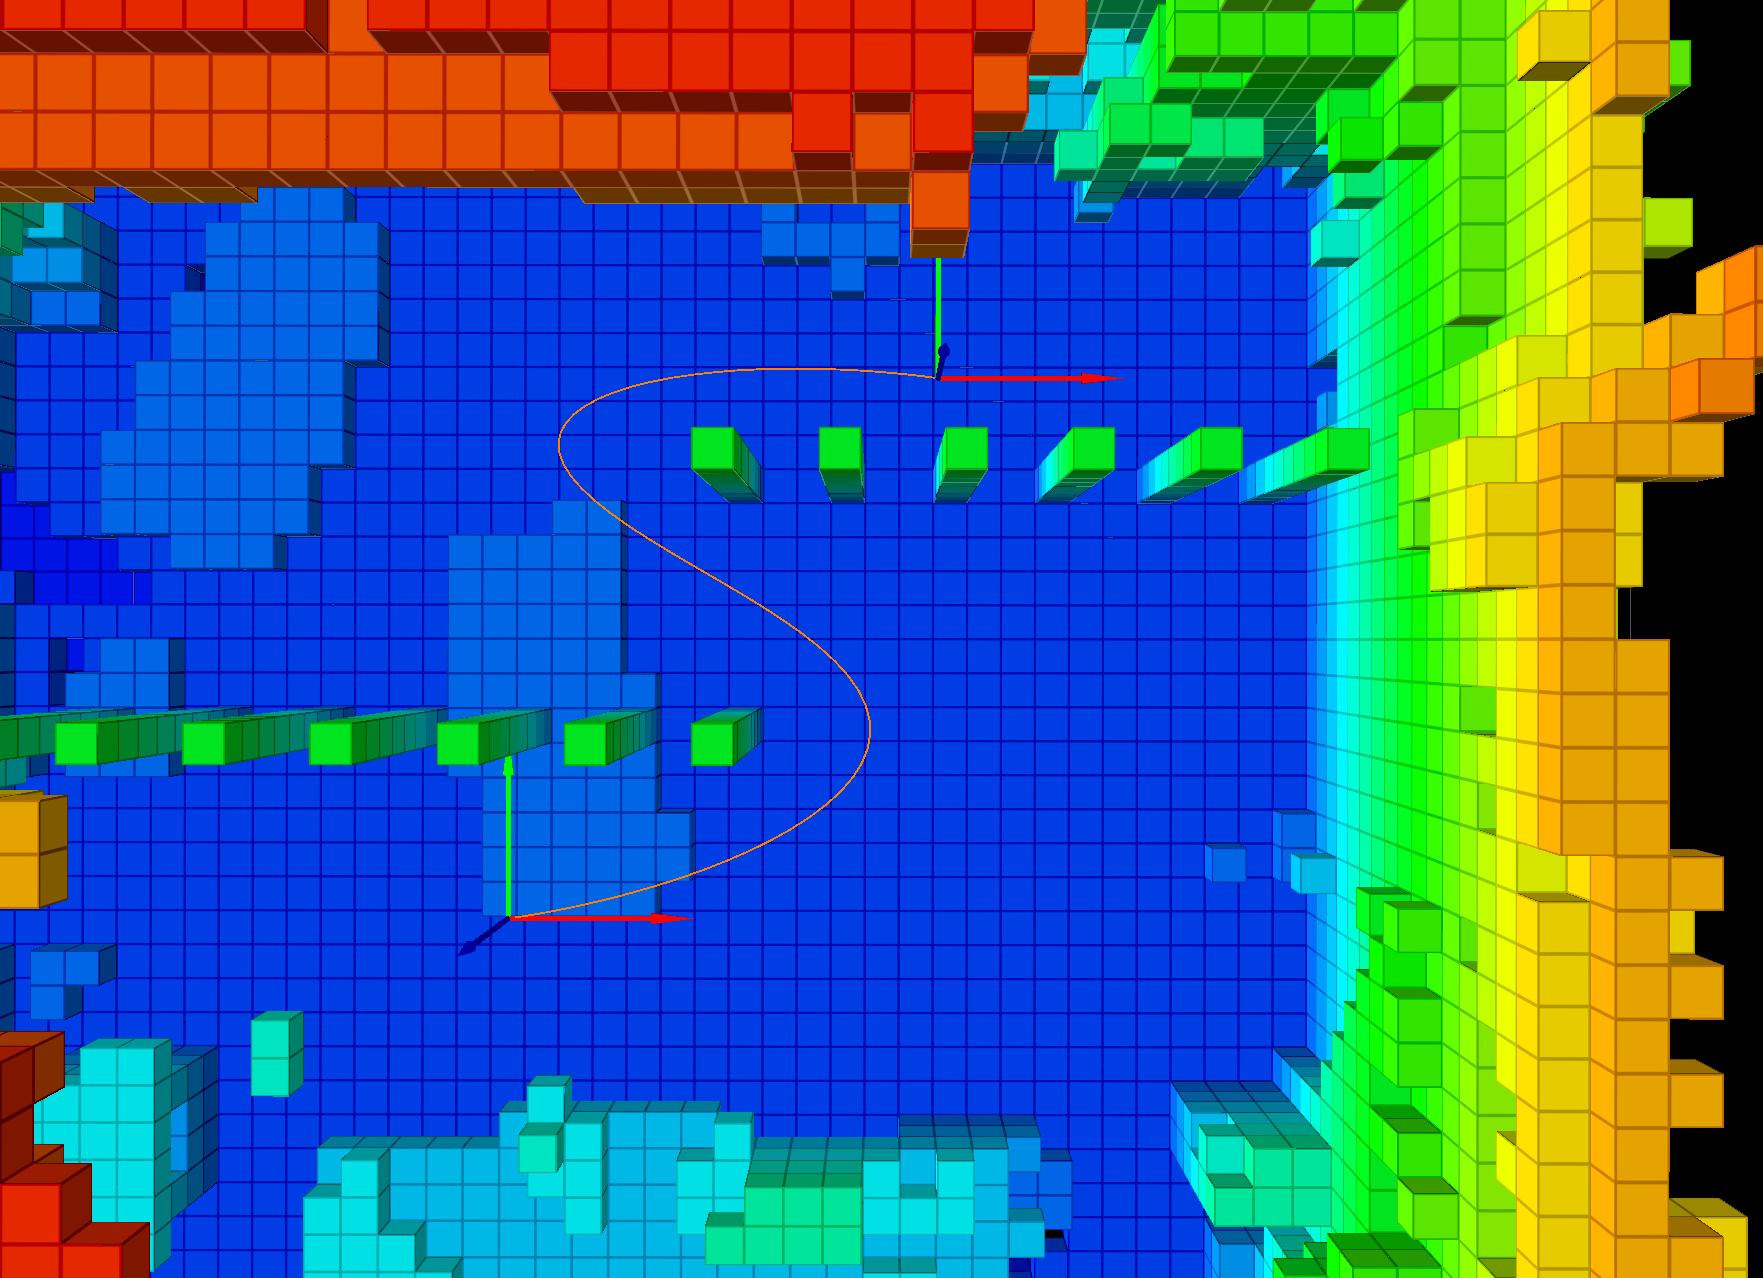
\includegraphics[width=1\linewidth]{pics/2b.png}
%  \caption{A subfigure}
%  \label{fig:sub2}
%\end{subfigure}
%\caption{A figure with two subfigures}
%\label{fig:testsdfaf}
%\end{figure}